%%% -*- coding: utf-8 -*-
\newpage

\chapter{Introduction}
\label{chap:introduction}

% INTRO SLR
The amount of multimedia content on the internet is increasing each year.
More than 300 hours of video are uploaded to YouTube every minute.\footnote{\url{https://biographon.com/youtube-stats}}
In this context, studies have shown that about 56\% of children between 10 and 13 years old have a smartphone \cite{remosoftware,chollet2017xception}, and 8 out of 10 teenagers have had a friend who shared some sensitive media through social networks such as Facebook, Twitter, and Whatsapp.\footnote{https://www.netnanny.com/the-importance-of-parental-control/}


% In Brazil, the ``Cicarely case'' was an example that forced youtube to be blocked.\footnote{\url{http://g1.globo.com/Noticias/Tecnologia/0,,AA1412609-6174-363,00.html}}
% In our research, we are interested in helping to avoid scenarios where pornography can be uploaded to education channels, which might expose students, sometimes underage, to this kind of content.\footnote{\url{https://g1.globo.com/sp/sao-paulo/noticia/2020/06/19/professor-de-etec-na-zona-norte-de-sp-e-afastado-apos-se-masturbar-durante-aula-virtual.ghtml}}. 
%This scenery presents challenges on controlling which kind of contents are uploaded to this storage and distribution services, while dealing with great amounts of videos.

This huge amount of data sharing pattern presents a challenge to the control of the type of content that is loaded to these video repositories. By allowing the upload of sensitive content from malicious users, content providers become exposed to legal issues. This is also a problem for users in those platforms, as they might get exposed to this content without a warning.

Methods based on \textit{Deep Learning} (DL) became the \textit{state-of-the-art} in various segments related to automatic video analysis. More specifically, 
Convolutional Neural Networks (CNN) architectures, or ConvNets, have become the primary method used for audio-visual pattern recognition.

The term \emph{Sensitive content} is often used as a reference to any media that contains content such as nudity, intense sexuality, violence, gore, and any other potentially disturbing or offensive subject.
On the other hand, a content is labeled as \emph{Safe} when that content is suitable for the general public.


% \begin{figure}[!ht]
%   \centering
%   \begin{subfigure}[b]{0.45\textwidth}
%     \centering
%     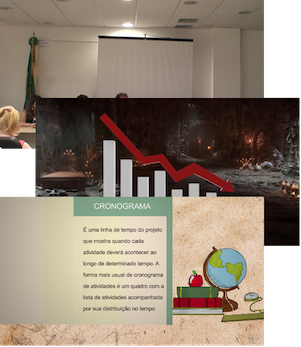
\includegraphics[width=0.8\textwidth]{img/safe.png}
%     \subcaption{Safe videos.}
%     \label{fig:samples_safe}
%   \end{subfigure}
%   \hspace{2em}
%   \begin{subfigure}[b]{0.45\textwidth}
%     \centering
%     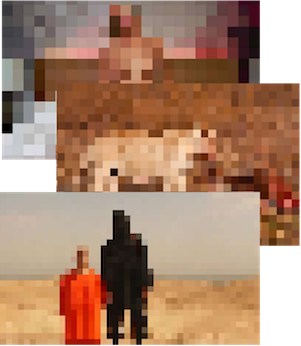
\includegraphics[width=0.8\textwidth]{img/sensitive.png}
%     \subcaption{Sensitive videos }
%     \label{fig:samples_not_save}
%   \end{subfigure}
%   \caption{Examples of Safe and Sensitive content.}
%   \label{fig:samples}
% \end{figure}
\begin{figure*}[!ht]
    \centering
    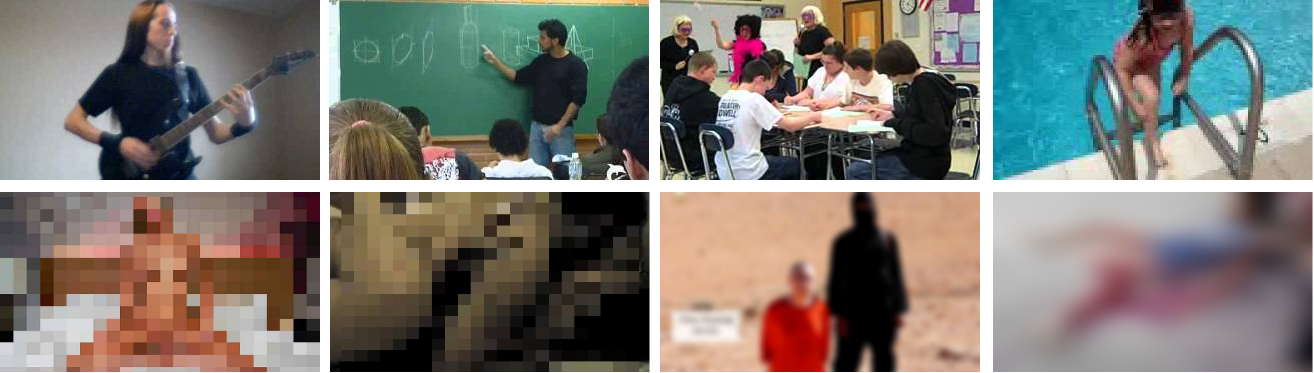
\includegraphics[width=0.95\textwidth]{img/safe-sensitive-horizontal.png}
    \caption{Examples of safe (top row) and sensitive videos (bottom row).}
    \label{fig:samples}
    \vspace{-1em}
\end{figure*}

Figure \ref{fig:samples} illustrates these two categories.
There are four scenes with safe content on the top row, and four scenes with sensitive content on the bottom row.

%As anyone can easily access any content on the Internet, whether exploring on search engines or through social networks, some groups of people (especially children) are very vulnerable to the exposure of content not suitable for their ages. 
%This situation calls for some media control strategy managed by parents or tutors, ensuring the least exposure to sensitive content.

%Controlling the type of content uploaded to video storage services requires an automatic analysis in an accurate and efficient way. 

%In this work, we created a CNN based model for video feature extraction and validate these video features experimenting with different baseline models to detect sensitive content.
%Then we evaluate the best model in a dataset created with videos sampled from the Brazilian RNP (National Research Network) repository video@RNP.\footnote{\url{https://www.video.rnp.br}}
%In our experimentation, the best model achieves a recall of 94.4\% and an F1-score of 95.6\% for pornography class.

Other works, such as \cite{moreira2019multimodal}, share our motivations and objectives, as described in Section \ref{chap:related}. However, most of them do not use both audio and image for classification. Some use hand-crafted feature extraction methods instead of more recent CNNs that has been showing great potential in video recognition and classification.

Our work uses two CNNs: one to extract image sequence features and the other to extract audio features.
As we get one feature vector for each second of the video, we can approach the feature classification task as a time series classification, using a Recurrent Neural Network (RNN) as baseline. We also can combine those features to create a single feature vector for the entire video, which then is used as the input for other baseline classifiers.
%Our method uses a rather simpler approach for video classification and yet it still yields results significantly close to related works.


%\todo{Also talk about scene localization, scene detection}

%What is the difference between sensitive content detection and classification?

Although the term \textit{classification} can be used to define the task we are addressing, in this work we favor the term \textit{detection} over \textit{classification} to avoid leaving an open interpretation, as the term \textit{classification} is often used to include tasks with multiple classes, while our task relies specifically on binary classification. Furthermore, \textit{Detection} in this context should not be interpreted as the task to find (either time-wise or space-wise) voice content in the video.
We use detection in a more specific sense: the act of finding out if sensitive media is or is not present in the content. 

%investigar a classifciacao e conteudo sensivel em video, principalmente em videos pornograficos e vi9lencia extrema

%objetivos espcificos
%cricao de dataset
%implemwentacao de baselines
%testar a eficiencia da extracao de features ja usada no yt8m
% testar a multimodalidade
% testar abordagem sequencial e não sequencial



%colocar exelpos do que é gore e oq n é 

%Obrigado pela recomendação professora! Foram excelentes leituras e tentarei trazer alguns desses conceitos para o meu trabalho.
% Infelizmente acho que nenhum dos datasets, apesar de numerosos e variados, é compativel com a nossa definição,

% O dataset que mais se aproximou com a nossa definição foi o MediaEval 2015, porém nosso dataset vem de principalmente de gravações amadoras ou CCTV, não de cenas cinematográficas.
% Seria interessante se testar se o treino em cenas amadoras se traduzem em bons resultados em cenas de estúdio, porém para fazer isso teriamos que filtrar alguns vídeos desse dataset que não entram em nossa definição.

% As nossas definições de violência são os vídeos de extremamente violentos (gore), que incluem pelo menos um desses: Sangue, Multilação e Morte.
% Não fazem parte da nossa definição: presença de armas, lutas, discussões, acidentes de carro (que não contenham nenhum dos topicos acima), violência emocional/mental e violência animada/cartunizada.

%In this work our goal is to create and validate a approach for sensitive content detection in video.

% Some of the questions we aim to answer with this work are:
% \begin{enumerate}
%     \item How does this approach compares with the related work?
%     \item What is the impact of also using audio in the model's performance?
%     \item Can the same model have a performance higher than 90\% on both pornography and violence detection tasks?
% \end{enumerate}

%To find the answers to these questions and fulfil our goal, 
The main contributions of this work are:
\begin{enumerate}
    % Criamos um dataset para a tarefa de classificacao de conteudo sensivel, o maior do mundo até onde sabemos
    \item To our knowledge, the largest sensistive content detection dataset.
    \item To our knowledge, we have obtained the best results in this task using only a generalistic feature extraction method and generic classifiers.
    % Testamos baselines nessa tarefa para validar o dataset e o funcionamento da extração de features
    \item We trained and tested baseline classifiers on the features extracted from our dataset in order to validate both the dataset and the efficiency nad operation of the genralistic feature extraction networks.  
    % Experimentamos com diferentes configurações de classificadores, inculsive sequenciais e naõ sequenciais
    \item We compared sequential and non sequential classifiers in this task.
    % Testamos a importancia dos features de imagem e de audio separadamente
    \item We tested the importance of image and audio features in this task.
    \item We also validate our approach by testing our best baseline in a well known pornography detection dataset, 2k-pornography. 
\end{enumerate}
Although the largest dataset for this task by our knowledge, our dataset is not manually labeled, which begs the question if it is noise-less enough for any training and evaluation in this task.  
Our intent is not to replace the 2k-pornography dataset, but to be a complement it, it still is the gold standard for pornography detection, in our dataset the videos were not manually labeled by a human, so we need to validate this dataset.

To perform this task, we created a large scale dataset, extracted features from this dataset using an generalist and well known feature extraction for video classification method, and performed experiments such as compare baseline classification models, compare which type of classification model (sequential or not) performs best, and compared the importance of audio and image features, further detailed in Chapter \ref{chap:method}.

This dissertation is organized as follows:
In Chapter \ref{chap:related} we discuss some of the related work.
\pva{TALVEZ INCLUIR THEORY?}
Then, in Chapter \ref{chap:method}, we detail our dataset and the proposed method to detect sensitive content in videos.
We present our dataset and metrics in Chapter \ref{chap:dataset}.
Then, we evaluate and analyse our baseline models in Chapter \ref{chap:results}.
Finally, in Chapter \ref{chap:conclusions} we present, our conclusions, currently published papers, and future work.
Additionaly, in Appendix \ref{chap:appendix}, we show complementary data, such as tables, distributions and a dataset datasheet.